% UIR-2 report, variant 51/51/30. Compile with XeLaTeX:  xelatex report.tex (twice)
\documentclass[12pt,a4paper]{article}
\usepackage{fontspec}
\usepackage{polyglossia}
\setdefaultlanguage{russian}
\setotherlanguage{english}
\IfFontExistsTF{Times New Roman}{\setmainfont{Times New Roman}}{\setmainfont{Liberation Serif}}
\IfFontExistsTF{Courier New}{\setmonofont{Courier New}[Scale=0.9]}{\setmonofont{Liberation Mono}[Scale=0.9]}
\usepackage[left=25mm,right=15mm,top=20mm,bottom=20mm]{geometry}
\usepackage{amsmath,amssymb}
\usepackage{graphicx,float,caption,subcaption}
\usepackage{booktabs,multirow,array,longtable,multicol}
\usepackage{tikz}
\usetikzlibrary{arrows.meta,positioning,fit}
\usepackage{indentfirst}
\usepackage{listings,xcolor}
\usepackage[hidelinks]{hyperref}
\captionsetup{labelsep=endash}
\setlength{\parskip}{3pt}
\linespread{1.1}
\emergencystretch=3em
\tolerance=2000
\lstset{basicstyle=\ttfamily\footnotesize, breaklines=true, frame=single, columns=fullflexible,
        showstringspaces=false, keywordstyle=\color{blue!60!black}, commentstyle=\color{gray}, language=Python}

\makeatletter\newcommand{\tabinput}[1]{\@@input #1 }\makeatother
\newcommand{\SoneThr}{0{,}1890}
\newcommand{\StwoThr}{0{,}1000}
\newcommand{\Ratio}{1{,}89}
\newcommand{\SonePi}{0{,}6220}
\newcommand{\StwoPi}{0{,}8000}
\newcommand{\SoneU}{25{,}06}
\newcommand{\StwoU}{37{,}88}
\newcommand{\SoneL}{2{,}846}
\newcommand{\StwoL}{2{,}788}
\newcommand{\SoneRho}{0{,}9451}
\newcommand{\StwoRho}{0{,}99996}
\newcommand{\SoneR}{1{,}8901}
\newcommand{\SoneThrA}{0{,}0980}
\newcommand{\SoneThrB}{0{,}0910}
\newcommand{\SonePiA}{0{,}6986}
\newcommand{\SonePiB}{0{,}4797}
\newcommand{\StwoExpThr}{0{,}0999}
\newcommand{\StwoExpU}{37{,}56}
\newcommand{\SoneSymThr}{0{,}1921}
\newcommand{\SoneZero}{0{,}001822}
\newcommand{\StwoZero}{0{,}000036}
\newcommand{\SoneFull}{0{,}335118}
\newcommand{\StwoFullSum}{0{,}8000}
\newcommand{\SoneMaxRes}{4{,}5\cdot10^{-17}}
\newcommand{\StwoMaxRes}{5{,}3\cdot10^{-17}}
% ---------- transition graph of SYSTEM_1 ----------
\newcommand{\graphOne}{%
\begin{tikzpicture}[>=Stealth, st/.style={circle, draw, thick, minimum size=10mm, inner sep=0pt, font=\small},
  lab/.style={font=\scriptsize, fill=white, inner sep=1pt}, x=2.75cm, y=2.15cm]
\foreach \a in {0,...,3}{\foreach \c in {0,...,3}{
  \pgfmathtruncatemacro{\k}{\a*4+\c+1}
  \node[st] (s\a\c) at (\c,-\a) {\a\c};
  \node[font=\tiny, text=gray, above left=-1.5mm and -1.5mm of s\a\c] {$E_{\k}$};
}}
\foreach \a in {0,...,3}{\foreach \c [evaluate=\c as \cn using int(\c+1)] in {0,1,2}{
  \draw[->] (s\a\c) to[bend left=18] node[lab, above]{$\lambda_2$} (s\a\cn);
  \draw[->] (s\a\cn) to[bend left=18] node[lab, below]{$\mu$} (s\a\c);
}}
\foreach \c in {0,...,3}{\foreach \a [evaluate=\a as \an using int(\a+1)] in {0,1,2}{
  \draw[->] (s\a\c) to[bend right=18] node[lab, left]{$\lambda_1$} (s\an\c);
  \draw[->] (s\an\c) to[bend right=18] node[lab, right]{$\mu$} (s\a\c);
}}
\end{tikzpicture}}

% ---------- transition graph of SYSTEM_2 ----------
\newcommand{\graphTwo}{%
\begin{tikzpicture}[>=Stealth, st/.style={circle, draw, thick, minimum size=10mm, inner sep=0pt, font=\small},
  lab/.style={font=\scriptsize, fill=white, inner sep=1pt}, x=3.1cm, y=2.3cm]
\node[st] (s0) at (0,-1) {$0$};
\node[font=\tiny, text=gray, above left=-1.5mm and -1.5mm of s0] {$E_{1}$};
\foreach \n in {1,...,4}{\foreach \j in {1,2,3}{
  \pgfmathtruncatemacro{\k}{(\n-1)*3+\j+1}
  \node[st] (s\n\j) at (\j,-\n) {$\n_{\j}$};
  \node[font=\tiny, text=gray, above left=-1.5mm and -1.5mm of s\n\j] {$E_{\k}$};
}}
% phase transitions
\foreach \n in {1,...,4}{
  \draw[->] (s\n1) -- node[lab, above]{$3\mu$} (s\n2);
  \draw[->] (s\n2) -- node[lab, above]{$3\mu$} (s\n3);
}
% arrivals
\draw[->] (s0) -- node[lab, above]{$\lambda$} (s11);
\foreach \j in {1,2,3}{\foreach \n [evaluate=\n as \nn using int(\n+1)] in {1,2,3}{
  \draw[->] (s\n\j) -- node[lab, left]{$\lambda$} (s\nn\j);
}}
% departures (end of phase 3)
\draw[->] (s13) to[out=150, in=60, looseness=0.9] node[lab, above]{$3\mu$} (s0);
\foreach \n [evaluate=\n as \np using int(\n-1)] in {2,3,4}{
  \draw[->, densely dashed] (s\n3) to[out=135, in=-20, looseness=0.6] node[lab, pos=0.45]{$3\mu$} (s\np1);
}
\end{tikzpicture}}

% ---------- structural schemes ----------
\newcommand{\schemeOne}{%
\begin{tikzpicture}[>=Stealth, font=\small,
  srv/.style={circle, draw, thick, minimum size=9mm}, buf/.style={rectangle, draw, minimum width=5mm, minimum height=6mm}]
\node (src) at (0,0) {$\lambda$};
\node[circle, fill, inner sep=1.5pt] (sp) at (1.4,0) {};
\draw[->] (src) -- (sp);
\foreach \y/\i/\q in {0.9/1/q_1, -0.9/2/q_2}{
  \node[buf] (b\i a) at (3.2,\y) {}; \node[buf, right=0pt of b\i a] (b\i b) {};
  \node[srv] (p\i) at (5.0,\y) {П\i};
  \draw[->] (sp) |- node[pos=0.75, above, font=\scriptsize]{$\q\lambda$} (b\i a.west);
  \draw[->] (b\i b) -- (p\i); \draw[->] (p\i) -- ++(1.1,0) node[right]{};
  \node[above=0pt of b\i a.north east, font=\scriptsize] {ЕН=2};
  \draw[->, gray] (b\i a.south west) ++(0,0) -- ++(-0.3,-0.35) node[below, font=\scriptsize]{потери};
}
\node[right, font=\scriptsize] at (6.1,0) {$b=10$ с, экспон.};
\end{tikzpicture}}

\newcommand{\schemeTwo}{%
\begin{tikzpicture}[>=Stealth, font=\small,
  ph/.style={rectangle, draw, thick, minimum width=8mm, minimum height=7mm}, buf/.style={rectangle, draw, minimum width=5mm, minimum height=6mm}]
\node (src) at (0,0) {$\lambda$};
\node[buf] (b1) at (1.6,0) {}; \node[buf, right=0pt of b1] (b2) {}; \node[buf, right=0pt of b2] (b3) {};
\node[above=0pt of b2.north, font=\scriptsize] {ЕН=3};
\node[ph] (f1) at (4.0,0) {Ф1}; \node[ph, right=4mm of f1] (f2) {Ф2}; \node[ph, right=4mm of f2] (f3) {Ф3};
\node[draw, dashed, rounded corners, fit=(f1)(f3), inner sep=3mm, label={above:{П ($E_3$): $b'=b/3$ на фазу}}] {};
\draw[->] (src) -- (b1); \draw[->] (b3) -- (f1); \draw[->] (f1) -- (f2); \draw[->] (f2) -- (f3); \draw[->] (f3) -- ++(1.1,0);
\draw[->, gray] (b1.south west) -- ++(-0.3,-0.35) node[below, font=\scriptsize]{потери};
\end{tikzpicture}}


\begin{document}
% ======================= TITLE =======================
\begin{titlepage}
\centering
{\large Университет ИТМО\\Факультет программной инженерии и компьютерной техники\par}
\vspace{5cm}
{\Large Дисциплина «Моделирование»\par}
\vspace{1cm}
{\LARGE\bfseries Учебно-исследовательская работа №\,2\par}
\vspace{0.4cm}
{\Large «Марковские модели систем массового обслуживания»\par}
\vspace{0.6cm}
{\large Вариант 51/51/30\par}
\vfill
\begin{flushright}
\begin{tabular}{l}
Выполнил: студент группы P3330\\
Рахаман Мд Афифур\\[4mm]
Преподаватель: Авксентьева Елена Юрьевна\\
\end{tabular}
\end{flushright}
\vspace{2cm}
Санкт-Петербург, 2026
\end{titlepage}

\tableofcontents
\newpage

% ======================= 1 =======================
\section{Цель работы и постановка задачи}
\textbf{Цель:} изучение метода марковских случайных процессов и его применение для исследования
систем массового обслуживания (СМО) с однородным потоком заявок.

\textbf{Задача:} разработать марковские модели двух вариантов организации СМО (СИСТЕМА\_1 и СИСТЕМА\_2),
рассчитать стационарные вероятности состояний и характеристики функционирования,
сравнить системы и выбрать лучшую по заданному критерию эффективности.

\subsection{Исходные данные}
Вариант задания: $N1/N2/NG = 51/51/30$.

\begin{table}[H]
\centering
\caption{Параметры структурной и функциональной организации (табл.\,1 задания)}
\begin{tabular}{cccccc}
\toprule
Вариант 1 & \multicolumn{2}{c}{СИСТЕМА\_1} & Вариант 2 & \multicolumn{2}{c}{СИСТЕМА\_2} \\
 & П & ЕН & & П & ЕН \\
\midrule
51 & 2 & 2/2 & 51 & 1 ($E_3$) & 3 \\
\bottomrule
\end{tabular}
\end{table}

\begin{table}[H]
\centering
\caption{Параметры нагрузки (табл.\,2 задания, группа 30)}
\begin{tabular}{cccccc}
\toprule
$\lambda$, 1/с & $b$, с & $\mu=1/b$, 1/с & П1 & П2 & П3 \\
\midrule
0,5 & 10 & 0,1 & 0,65 & 0,2 & 0,15 \\
\bottomrule
\end{tabular}
\end{table}

Вероятности занятия приборов:
\begin{itemize}
\item СИСТЕМА\_1 (двухканальная): $q_1 = 0{,}65$, \ $q_2 = 0{,}2 + 0{,}15 = 0{,}35$;
\item СИСТЕМА\_2 (одноканальная): $q = 1$.
\end{itemize}

\textbf{Критерий эффективности.} Так как $N1 + N2 = 51 + 51 = 102$~--- чётное число,
критерий выбирается по варианту $N2 = 51$: \textbf{(а) максимальная производительность системы}.

Суммарная нагрузка: $Y = \lambda b = 0{,}5\cdot 10 = 5$, т.\,е. обе системы работают в режиме
сильной перегрузки; стационарный режим существует, так как ёмкости накопителей ограничены.

% ======================= 2 =======================
\section{Описание исследуемых систем}
\subsection{СИСТЕМА\_1}
\begin{figure}[H]\centering\schemeOne\caption{Структура СИСТЕМЫ\_1}\end{figure}
\begin{itemize}
\item два обслуживающих прибора П1 и П2, длительность обслуживания в каждом распределена экспоненциально со средним $b = 10$ с ($\mu = 0{,}1$ 1/с);
\item перед каждым прибором свой накопитель ёмкостью 2 (ЕН\,=\,2/2);
\item входящий поток пуассоновский с интенсивностью $\lambda = 0{,}5$ 1/с; поступившая заявка с вероятностью $q_1 = 0{,}65$ направляется к П1 ($\lambda_1 = q_1\lambda = 0{,}325$ 1/с) и с вероятностью $q_2 = 0{,}35$~--- к П2 ($\lambda_2 = q_2\lambda = 0{,}175$ 1/с);
\item если накопитель выбранного прибора заполнен, заявка теряется (к другому прибору не переходит);
\item дисциплина обслуживания в очереди~--- FIFO, без приоритетов.
\end{itemize}
Так как разбиение пуассоновского потока даёт независимые пуассоновские потоки, каждая подсистема
«накопитель + прибор» ведёт себя как СМО M/M/1/3, однако в работе рассматривается общий марковский
процесс для всей системы.

\subsection{СИСТЕМА\_2}
\begin{figure}[H]\centering\schemeTwo\caption{Структура СИСТЕМЫ\_2}\end{figure}
\begin{itemize}
\item один обслуживающий прибор, длительность обслуживания распределена по закону Эрланга 3-го порядка со средним $b = 10$ с (коэффициент вариации $\nu = 1/\sqrt{3} \approx 0{,}577$);
\item общий накопитель ёмкостью 3; всего в системе может находиться не более 4 заявок;
\item входящий поток пуассоновский, $\lambda = 0{,}5$ 1/с; заявка, заставшая накопитель заполненным, теряется.
\end{itemize}

\textbf{Сведение к марковскому процессу.} Процесс в СИСТЕМЕ\_2 не является марковским, так как длительность
обслуживания не экспоненциальна. Используется представление закона Эрланга 3-го порядка суммой трёх
экспоненциально распределённых фаз Ф1, Ф2, Ф3 со средним $b' = b/3 = 10/3$ с каждая, т.\,е.
интенсивность прохождения фазы $3\mu = 0{,}3$ 1/с. Тогда процесс с состояниями, учитывающими номер
текущей фазы обслуживания, является марковским.

% ======================= 3 =======================
\section{Кодирование и перечень состояний}
\subsection{СИСТЕМА\_1}
Состояние кодируется парой $(n_1 n_2)$, где $n_i \in \{0,1,2,3\}$~--- число заявок у прибора П$i$
(одна на обслуживании и до двух в накопителе). Число состояний $4\cdot 4 = 16 \le 20$, поэтому
изменение параметров системы не требуется.

\begin{table}[H]
\centering\small
\caption{Перечень состояний СИСТЕМЫ\_1}
\begin{tabular}{cc l}
\toprule
Сост. & Код $(n_1 n_2)$ & Описание \\
\midrule
$E_1$ & 00 & система пуста \\
$E_2$–$E_4$ & 01, 02, 03 & П1 свободен; у П2 1, 2, 3 заявки \\
$E_5$–$E_8$ & 10, 11, 12, 13 & П1 обслуживает 1 заявку, очередь к П1 пуста \\
$E_9$–$E_{12}$ & 20, 21, 22, 23 & П1 занят, в накопителе П1 одна заявка \\
$E_{13}$–$E_{16}$ & 30, 31, 32, 33 & П1 занят, накопитель П1 заполнен (2 заявки) \\
\bottomrule
\end{tabular}
\end{table}
В общем виде: состояние $(n_1 n_2)$ имеет номер $E_{4n_1+n_2+1}$; $n_i=0$~--- прибор П$i$ свободен,
$n_i\ge1$~--- прибор занят и в его накопителе $n_i-1$ заявок; $n_i=3$~--- накопитель заполнен,
заявки, направляемые к П$i$, теряются.

\subsection{СИСТЕМА\_2}
Состояние кодируется как $0$ (система пуста) или $n_j$, где $n \in \{1,2,3,4\}$~--- общее число заявок в
системе (одна на обслуживании, $n-1$ в накопителе), $j\in\{1,2,3\}$~--- номер фазы распределения Эрланга,
на которой находится обслуживаемая заявка. Число состояний $1 + 4\cdot3 = 13 \le 20$.

\begin{table}[H]
\centering\small
\caption{Перечень состояний СИСТЕМЫ\_2}
\begin{tabular}{ccl}
\toprule
Сост. & Код & Описание \\
\midrule
$E_1$ & 0 & система пуста \\
$E_2,E_3,E_4$ & $1_1, 1_2, 1_3$ & 1 заявка на обслуживании (фаза 1, 2, 3), накопитель пуст \\
$E_5,E_6,E_7$ & $2_1, 2_2, 2_3$ & 1 заявка на обслуживании, 1 в накопителе \\
$E_8,E_9,E_{10}$ & $3_1, 3_2, 3_3$ & 1 заявка на обслуживании, 2 в накопителе \\
$E_{11},E_{12},E_{13}$ & $4_1, 4_2, 4_3$ & 1 заявка на обслуживании, 3 в накопителе (заполнен) \\
\bottomrule
\end{tabular}
\end{table}

% ======================= 4 =======================
\section{Размеченные графы переходов}
\subsection{СИСТЕМА\_1}
Переходы: поступление заявки к П1 ($n_1\to n_1+1$, интенсивность $\lambda_1$, если $n_1<3$),
поступление заявки к П2 ($n_2\to n_2+1$, $\lambda_2$, если $n_2<3$), завершение обслуживания
в П1 или П2 ($n_i\to n_i-1$, интенсивность $\mu$, если $n_i>0$).
\begin{figure}[H]
\centering
\resizebox{0.92\textwidth}{!}{\graphOne}
\caption{Размеченный граф переходов СИСТЕМЫ\_1 ($\lambda_1=0{,}325$, $\lambda_2=0{,}175$, $\mu=0{,}1$ 1/с); строка~--- $n_1$, столбец~--- $n_2$}
\end{figure}

\subsection{СИСТЕМА\_2}
Переходы: поступление заявки ($n_j \to (n+1)_j$, интенсивность $\lambda$, если $n<4$; из $0$ в $1_1$),
переход к следующей фазе обслуживания ($n_j \to n_{j+1}$, $3\mu$), завершение обслуживания после третьей
фазы ($n_3 \to (n-1)_1$ или $1_3 \to 0$, $3\mu$)~--- на обслуживание сразу поступает следующая заявка из накопителя
и начинает с первой фазы.
\begin{figure}[H]
\centering
\resizebox{0.85\textwidth}{!}{\graphTwo}
\caption{Размеченный граф переходов СИСТЕМЫ\_2 ($\lambda=0{,}5$, $3\mu=0{,}3$ 1/с); штриховые дуги~--- завершение обслуживания}
\end{figure}

% ======================= 5 =======================
\section{Матрицы интенсивностей переходов}
Элемент $g_{ij}$ ($i\ne j$)~--- интенсивность перехода из $E_i$ в $E_j$; диагональный элемент
$g_{ii} = -\sum_{j\ne i} g_{ij}$ (выделен жирным). Пустые клетки~--- нули.
Стационарные вероятности находятся из системы
\[
\sum_{i} p_i\, g_{ij} = 0,\quad j=1,\dots,n; \qquad \sum_i p_i = 1 .
\]

\subsection{СИСТЕМА\_1}
\begin{table}[H]
\centering
\caption{Матрица интенсивностей переходов $G_1$ (16$\times$16)}
\setlength{\tabcolsep}{1.2pt}
\resizebox{\textwidth}{!}{\tiny\begin{tabular}{c|cccccccccccccccc}
 & $E_{1}$ & $E_{2}$ & $E_{3}$ & $E_{4}$ & $E_{5}$ & $E_{6}$ & $E_{7}$ & $E_{8}$ & $E_{9}$ & $E_{10}$ & $E_{11}$ & $E_{12}$ & $E_{13}$ & $E_{14}$ & $E_{15}$ & $E_{16}$ \\ \hline
$E_{1}$ & \textbf{-0{,}500} & 0{,}175 &  &  & 0{,}325 &  &  &  &  &  &  &  &  &  &  &  \\
$E_{2}$ & 0{,}100 & \textbf{-0{,}600} & 0{,}175 &  &  & 0{,}325 &  &  &  &  &  &  &  &  &  &  \\
$E_{3}$ &  & 0{,}100 & \textbf{-0{,}600} & 0{,}175 &  &  & 0{,}325 &  &  &  &  &  &  &  &  &  \\
$E_{4}$ &  &  & 0{,}100 & \textbf{-0{,}425} &  &  &  & 0{,}325 &  &  &  &  &  &  &  &  \\
$E_{5}$ & 0{,}100 &  &  &  & \textbf{-0{,}600} & 0{,}175 &  &  & 0{,}325 &  &  &  &  &  &  &  \\
$E_{6}$ &  & 0{,}100 &  &  & 0{,}100 & \textbf{-0{,}700} & 0{,}175 &  &  & 0{,}325 &  &  &  &  &  &  \\
$E_{7}$ &  &  & 0{,}100 &  &  & 0{,}100 & \textbf{-0{,}700} & 0{,}175 &  &  & 0{,}325 &  &  &  &  &  \\
$E_{8}$ &  &  &  & 0{,}100 &  &  & 0{,}100 & \textbf{-0{,}525} &  &  &  & 0{,}325 &  &  &  &  \\
$E_{9}$ &  &  &  &  & 0{,}100 &  &  &  & \textbf{-0{,}600} & 0{,}175 &  &  & 0{,}325 &  &  &  \\
$E_{10}$ &  &  &  &  &  & 0{,}100 &  &  & 0{,}100 & \textbf{-0{,}700} & 0{,}175 &  &  & 0{,}325 &  &  \\
$E_{11}$ &  &  &  &  &  &  & 0{,}100 &  &  & 0{,}100 & \textbf{-0{,}700} & 0{,}175 &  &  & 0{,}325 &  \\
$E_{12}$ &  &  &  &  &  &  &  & 0{,}100 &  &  & 0{,}100 & \textbf{-0{,}525} &  &  &  & 0{,}325 \\
$E_{13}$ &  &  &  &  &  &  &  &  & 0{,}100 &  &  &  & \textbf{-0{,}275} & 0{,}175 &  &  \\
$E_{14}$ &  &  &  &  &  &  &  &  &  & 0{,}100 &  &  & 0{,}100 & \textbf{-0{,}375} & 0{,}175 &  \\
$E_{15}$ &  &  &  &  &  &  &  &  &  &  & 0{,}100 &  &  & 0{,}100 & \textbf{-0{,}375} & 0{,}175 \\
$E_{16}$ &  &  &  &  &  &  &  &  &  &  &  & 0{,}100 &  &  & 0{,}100 & \textbf{-0{,}200} \\
\end{tabular}}
\end{table}
Ненулевые интенсивности (в форме, удобной для ввода в программу MARK):
\begin{multicols}{4}\footnotesize
$E_{1}\to E_{2}$: $\lambda_2=0{,}175$\\$E_{1}\to E_{5}$: $\lambda_1=0{,}325$\\$E_{2}\to E_{1}$: $\mu=0{,}100$\\$E_{2}\to E_{3}$: $\lambda_2=0{,}175$\\$E_{2}\to E_{6}$: $\lambda_1=0{,}325$\\$E_{3}\to E_{2}$: $\mu=0{,}100$\\$E_{3}\to E_{4}$: $\lambda_2=0{,}175$\\$E_{3}\to E_{7}$: $\lambda_1=0{,}325$\\$E_{4}\to E_{3}$: $\mu=0{,}100$\\$E_{4}\to E_{8}$: $\lambda_1=0{,}325$\\$E_{5}\to E_{1}$: $\mu=0{,}100$\\$E_{5}\to E_{6}$: $\lambda_2=0{,}175$\\$E_{5}\to E_{9}$: $\lambda_1=0{,}325$\\$E_{6}\to E_{2}$: $\mu=0{,}100$\\$E_{6}\to E_{5}$: $\mu=0{,}100$\\$E_{6}\to E_{7}$: $\lambda_2=0{,}175$\\$E_{6}\to E_{10}$: $\lambda_1=0{,}325$\\$E_{7}\to E_{3}$: $\mu=0{,}100$\\$E_{7}\to E_{6}$: $\mu=0{,}100$\\$E_{7}\to E_{8}$: $\lambda_2=0{,}175$\\$E_{7}\to E_{11}$: $\lambda_1=0{,}325$\\$E_{8}\to E_{4}$: $\mu=0{,}100$\\$E_{8}\to E_{7}$: $\mu=0{,}100$\\$E_{8}\to E_{12}$: $\lambda_1=0{,}325$\\$E_{9}\to E_{5}$: $\mu=0{,}100$\\$E_{9}\to E_{10}$: $\lambda_2=0{,}175$\\$E_{9}\to E_{13}$: $\lambda_1=0{,}325$\\$E_{10}\to E_{6}$: $\mu=0{,}100$\\$E_{10}\to E_{9}$: $\mu=0{,}100$\\$E_{10}\to E_{11}$: $\lambda_2=0{,}175$\\$E_{10}\to E_{14}$: $\lambda_1=0{,}325$\\$E_{11}\to E_{7}$: $\mu=0{,}100$\\$E_{11}\to E_{10}$: $\mu=0{,}100$\\$E_{11}\to E_{12}$: $\lambda_2=0{,}175$\\$E_{11}\to E_{15}$: $\lambda_1=0{,}325$\\$E_{12}\to E_{8}$: $\mu=0{,}100$\\$E_{12}\to E_{11}$: $\mu=0{,}100$\\$E_{12}\to E_{16}$: $\lambda_1=0{,}325$\\$E_{13}\to E_{9}$: $\mu=0{,}100$\\$E_{13}\to E_{14}$: $\lambda_2=0{,}175$\\$E_{14}\to E_{10}$: $\mu=0{,}100$\\$E_{14}\to E_{13}$: $\mu=0{,}100$\\$E_{14}\to E_{15}$: $\lambda_2=0{,}175$\\$E_{15}\to E_{11}$: $\mu=0{,}100$\\$E_{15}\to E_{14}$: $\mu=0{,}100$\\$E_{15}\to E_{16}$: $\lambda_2=0{,}175$\\$E_{16}\to E_{12}$: $\mu=0{,}100$\\$E_{16}\to E_{15}$: $\mu=0{,}100$
\end{multicols}

\subsection{СИСТЕМА\_2}
\begin{table}[H]
\centering
\caption{Матрица интенсивностей переходов $G_2$ (13$\times$13)}
\setlength{\tabcolsep}{2pt}
\resizebox{\textwidth}{!}{\scriptsize\begin{tabular}{c|ccccccccccccc}
 & $E_{1}$ & $E_{2}$ & $E_{3}$ & $E_{4}$ & $E_{5}$ & $E_{6}$ & $E_{7}$ & $E_{8}$ & $E_{9}$ & $E_{10}$ & $E_{11}$ & $E_{12}$ & $E_{13}$ \\ \hline
$E_{1}$ & \textbf{-0{,}500} & 0{,}500 &  &  &  &  &  &  &  &  &  &  &  \\
$E_{2}$ &  & \textbf{-0{,}800} & 0{,}300 &  & 0{,}500 &  &  &  &  &  &  &  &  \\
$E_{3}$ &  &  & \textbf{-0{,}800} & 0{,}300 &  & 0{,}500 &  &  &  &  &  &  &  \\
$E_{4}$ & 0{,}300 &  &  & \textbf{-0{,}800} &  &  & 0{,}500 &  &  &  &  &  &  \\
$E_{5}$ &  &  &  &  & \textbf{-0{,}800} & 0{,}300 &  & 0{,}500 &  &  &  &  &  \\
$E_{6}$ &  &  &  &  &  & \textbf{-0{,}800} & 0{,}300 &  & 0{,}500 &  &  &  &  \\
$E_{7}$ &  & 0{,}300 &  &  &  &  & \textbf{-0{,}800} &  &  & 0{,}500 &  &  &  \\
$E_{8}$ &  &  &  &  &  &  &  & \textbf{-0{,}800} & 0{,}300 &  & 0{,}500 &  &  \\
$E_{9}$ &  &  &  &  &  &  &  &  & \textbf{-0{,}800} & 0{,}300 &  & 0{,}500 &  \\
$E_{10}$ &  &  &  &  & 0{,}300 &  &  &  &  & \textbf{-0{,}800} &  &  & 0{,}500 \\
$E_{11}$ &  &  &  &  &  &  &  &  &  &  & \textbf{-0{,}300} & 0{,}300 &  \\
$E_{12}$ &  &  &  &  &  &  &  &  &  &  &  & \textbf{-0{,}300} & 0{,}300 \\
$E_{13}$ &  &  &  &  &  &  &  & 0{,}300 &  &  &  &  & \textbf{-0{,}300} \\
\end{tabular}}
\end{table}
Ненулевые интенсивности:
\begin{multicols}{4}\footnotesize
$E_{1}\to E_{2}$: $\lambda=0{,}500$\\$E_{2}\to E_{3}$: $3\mu=0{,}300$\\$E_{2}\to E_{5}$: $\lambda=0{,}500$\\$E_{3}\to E_{4}$: $3\mu=0{,}300$\\$E_{3}\to E_{6}$: $\lambda=0{,}500$\\$E_{4}\to E_{1}$: $3\mu=0{,}300$\\$E_{4}\to E_{7}$: $\lambda=0{,}500$\\$E_{5}\to E_{6}$: $3\mu=0{,}300$\\$E_{5}\to E_{8}$: $\lambda=0{,}500$\\$E_{6}\to E_{7}$: $3\mu=0{,}300$\\$E_{6}\to E_{9}$: $\lambda=0{,}500$\\$E_{7}\to E_{2}$: $3\mu=0{,}300$\\$E_{7}\to E_{10}$: $\lambda=0{,}500$\\$E_{8}\to E_{9}$: $3\mu=0{,}300$\\$E_{8}\to E_{11}$: $\lambda=0{,}500$\\$E_{9}\to E_{10}$: $3\mu=0{,}300$\\$E_{9}\to E_{12}$: $\lambda=0{,}500$\\$E_{10}\to E_{5}$: $3\mu=0{,}300$\\$E_{10}\to E_{13}$: $\lambda=0{,}500$\\$E_{11}\to E_{12}$: $3\mu=0{,}300$\\$E_{12}\to E_{13}$: $3\mu=0{,}300$\\$E_{13}\to E_{8}$: $3\mu=0{,}300$
\end{multicols}

% ======================= 6 =======================
\section{Стационарные вероятности состояний}
Стационарные вероятности получены решением системы линейных уравнений из п.\,5
(в программе MARK; для контроля система решена также численно в Python/NumPy, см. приложение~А).
Невязка $\max_j|\sum_i p_i g_{ij}|$ составляет $\SoneMaxRes$ для СИСТЕМЫ\_1 и $\StwoMaxRes$
для СИСТЕМЫ\_2, сумма вероятностей равна 1.

% If you have MARK screenshots, put them into figures/ and uncomment:
% \begin{figure}[H]\centering\includegraphics[width=0.8\textwidth]{figures/mark_sys1.png}\caption{Результаты MARK, СИСТЕМА\_1}\end{figure}
% \begin{figure}[H]\centering\includegraphics[width=0.8\textwidth]{figures/mark_sys2.png}\caption{Результаты MARK, СИСТЕМА\_2}\end{figure}

\begin{table}[H]
\centering
\caption*{\textit{Форма 1}}
\caption{Стационарные вероятности состояний}
\begin{tabular}{c|ll|ll}
\toprule
Номер & \multicolumn{2}{c|}{СИСТЕМА\_1} & \multicolumn{2}{c}{СИСТЕМА\_2} \\
состояния & Обозн. & Вер-ть & Обозн. & Вер-ть \\
\midrule
\tabinput{tex/form1.tex}
\bottomrule
\end{tabular}
\end{table}

Наиболее вероятное состояние СИСТЕМЫ\_1~--- $(33)$, оба накопителя заполнены
($p = \SoneFull$); вероятность простоя всей системы $p_{00} = \SoneZero$. В СИСТЕМЕ\_2 вероятность
того, что накопитель заполнен ($4_1+4_2+4_3$), равна $\StwoFullSum$, а вероятность простоя
$p_0 = \StwoZero$. Это закономерно при нагрузке $Y = 5$.

% ======================= 7 =======================
\section{Характеристики функционирования систем}
Обозначения: $p$~--- стационарная вероятность состояния, суммирование ведётся по состояниям,
удовлетворяющим указанному условию; $n_1, n_2$~--- число заявок у П1 и П2 (СИСТЕМА\_1),
$n$~--- число заявок в СИСТЕМЕ\_2; $(x)^+ = \max(x,0)$.
Все характеристики, кроме времён, рассчитаны непосредственно через вероятности состояний;
вероятность потери равна вероятности того, что накопитель выбранного прибора заполнен
(пуассоновский поток «видит» стационарное распределение).

\begin{table}[H]
\centering\small
\caption*{\textit{Форма 2}}
\caption{Характеристики систем}
\renewcommand{\arraystretch}{1.25}
\begin{tabular}{|>{\raggedright\arraybackslash}p{3.0cm}|>{\raggedright\arraybackslash}p{1.9cm}|c|c|r|r|}
\hline
Хар-ка & Прибор & Формула (СИСТ.\,1) & Формула (СИСТ.\,2) & СИСТ.\,1 & СИСТ.\,2 \\
\hline
\tabinput{tex/form2.tex}
\end{tabular}
\end{table}

Состояния с потерями: для П1 СИСТЕМЫ\_1~--- $n_1 = 3$ ($E_{13}$–$E_{16}$), для П2~--- $n_2 = 3$
($E_4, E_8, E_{12}, E_{16}$), для СИСТЕМЫ\_2~--- $n = 4$ ($E_{11}$–$E_{13}$). Загрузка СИСТЕМЫ\_1 приведена к одному прибору
($\rho = R/2$), а $R$~--- среднее число одновременно работающих приборов.

\subsection{Проверка результатов}
Проверка выполнена с помощью фундаментальных соотношений:
\begin{itemize}
\item производительность прибора равна $\lambda' = \rho/b$ (интенсивность выхода из работающего прибора);
\item $m = l + \rho$ (заявки в системе = в очереди + на обслуживании);
\item формула Литтла: $u = w + b$;
\item для СИСТЕМЫ\_2 дополнительно $\lambda' = 3\mu\,(p_{1_3}+p_{2_3}+p_{3_3}+p_{4_3})$;
\item для СИСТЕМЫ\_1: $\pi = q_1\pi_1 + q_2\pi_2$.
\end{itemize}

\begin{table}[H]
\centering\small
\caption{Проверка соотношений}
\begin{tabular}{lcccccc}
\toprule
Прибор & $\lambda'=\lambda(1-\pi)$ & $\rho/b$ & $u=m/\lambda'$ & $w+b$ & $m$ & $l+\rho$ \\
\midrule
\tabinput{tex/checks.tex}
\bottomrule
\end{tabular}
\end{table}
Все соотношения выполняются с точностью до погрешности округления, что подтверждает корректность
построенных моделей и рассчитанных вероятностей.

% ======================= 8 =======================
\section{Сравнительный анализ систем}
\subsection{При заданных параметрах ($\lambda=0{,}5$ 1/с, $b=10$ с)}
\begin{table}[H]
\centering
\caption{Сравнение основных характеристик}
\begin{tabular}{lccc}
\toprule
Характеристика & СИСТЕМА\_1 & СИСТЕМА\_2 & Лучше \\
\midrule
Производительность $\Lambda'$, 1/с & \SoneThr & \StwoThr & С1 (в \Ratio\ раза) \\
Вероятность потери $\pi$ & \SonePi & \StwoPi & С1 \\
Загрузка прибора $\rho$ & \SoneRho & \StwoRho & С2 \\
Ср. число работающих приборов $R$ & \SoneR & \StwoRho & С1 \\
Суммарная длина очередей $L$ & \SoneL & \StwoL & С2 (незначительно) \\
Время пребывания $U$, с & \SoneU & \StwoU & С1 \\
\bottomrule
\end{tabular}
\end{table}

\textbf{Выводы по сравнению.}
\begin{enumerate}
\item Производительность одноканальной СИСТЕМЫ\_2 ограничена сверху величиной $1/b = 0{,}1$ 1/с,
которая при нагрузке $Y=5$ практически достигнута ($\rho \approx 0{,}99996$). СИСТЕМА\_1 имеет два прибора,
поэтому её предельная производительность $2/b = 0{,}2$ 1/с; фактическое значение \SoneThr\ 1/с
в \Ratio\ раза больше, чем у СИСТЕМЫ\_2.
\item Потери в СИСТЕМЕ\_2 составляют 80\,\% против 62\,\% в СИСТЕМЕ\_1. В СИСТЕМЕ\_1 больше теряется
заявок, направленных к более нагруженному П1 ($\pi_1 = \SonePiA$ против $\pi_2 = \SonePiB$).
\item Загрузка одного прибора в СИСТЕМЕ\_2 выше (прибор почти никогда не простаивает), но это
следствие нехватки мощности, а не преимущество: суммарно в СИСТЕМЕ\_1 работает в среднем
\SoneR\ прибора.
\item Суммарная длина очередей почти одинакова (\SoneL\ и \StwoL), однако в СИСТЕМЕ\_1 очереди
обслуживаются двумя приборами параллельно, поэтому среднее время пребывания заявки
меньше в 1,5 раза (\SoneU\ с против \StwoU\ с).
\item Эрланговское обслуживание ($\nu\approx0{,}58$) при такой перегрузке почти не влияет на результат:
при экспоненциальном обслуживании в СИСТЕМЕ\_2 производительность была бы \StwoExpThr\ 1/с.
Определяющим фактором является число приборов.
\end{enumerate}

\subsection{Зависимость характеристик от интенсивности входящего потока}
Для анализа устойчивости вывода интенсивность $\lambda$ варьировалась в диапазоне $0{,}01$–$1$ 1/с
при неизменных остальных параметрах (рис.\,\ref{fig:thr}–\ref{fig:m}).

\begin{figure}[H]
\centering
\begin{subfigure}{0.49\textwidth}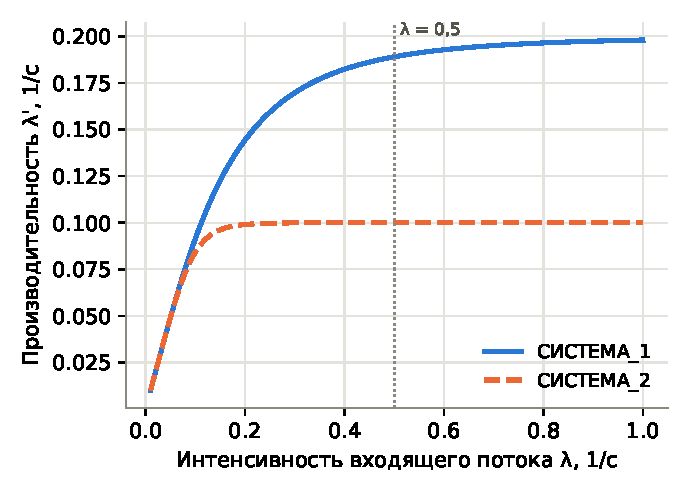
\includegraphics[width=\linewidth]{figures/thr.pdf}\caption{Производительность}\label{fig:thr}\end{subfigure}
\begin{subfigure}{0.49\textwidth}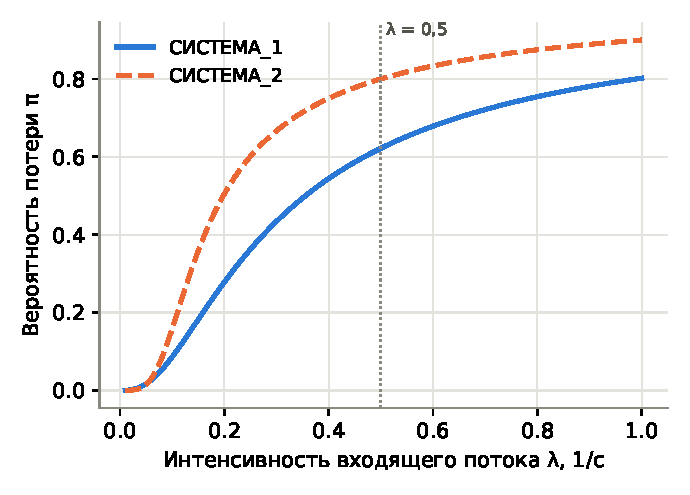
\includegraphics[width=\linewidth]{figures/loss.pdf}\caption{Вероятность потери}\end{subfigure}
\begin{subfigure}{0.49\textwidth}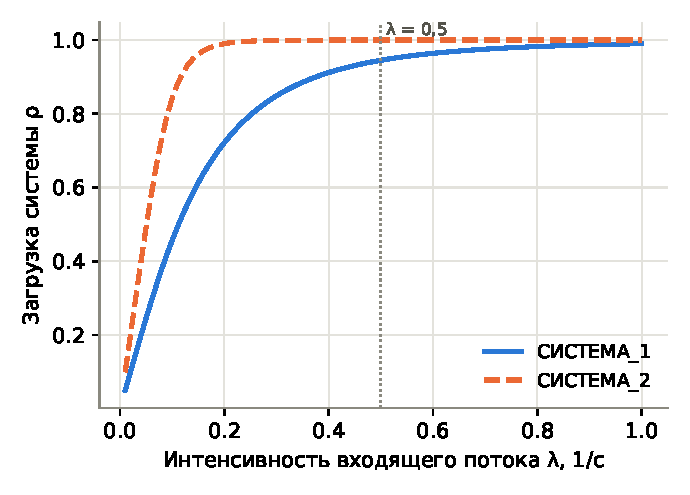
\includegraphics[width=\linewidth]{figures/rho.pdf}\caption{Загрузка}\end{subfigure}
\begin{subfigure}{0.49\textwidth}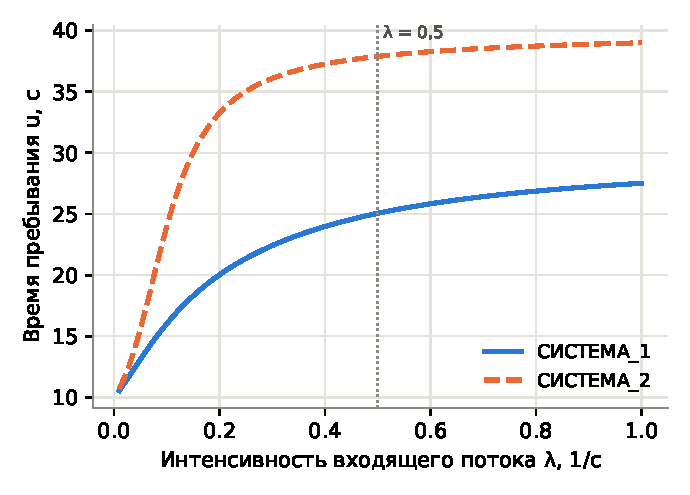
\includegraphics[width=\linewidth]{figures/u.pdf}\caption{Время пребывания}\end{subfigure}
\begin{subfigure}{0.49\textwidth}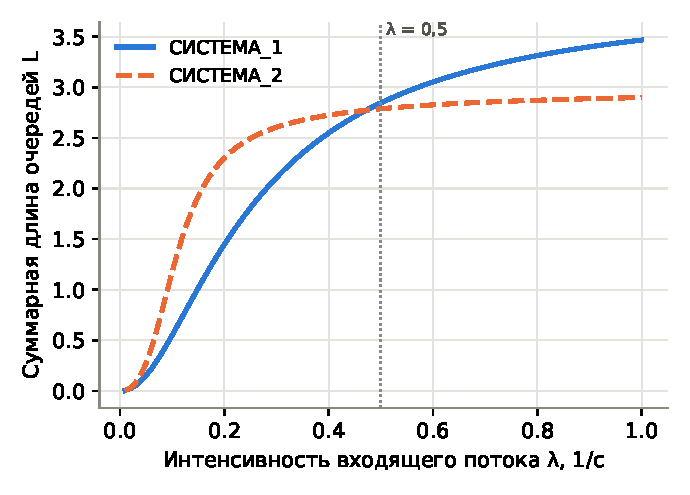
\includegraphics[width=\linewidth]{figures/queue.pdf}\caption{Суммарная длина очередей}\end{subfigure}
\begin{subfigure}{0.49\textwidth}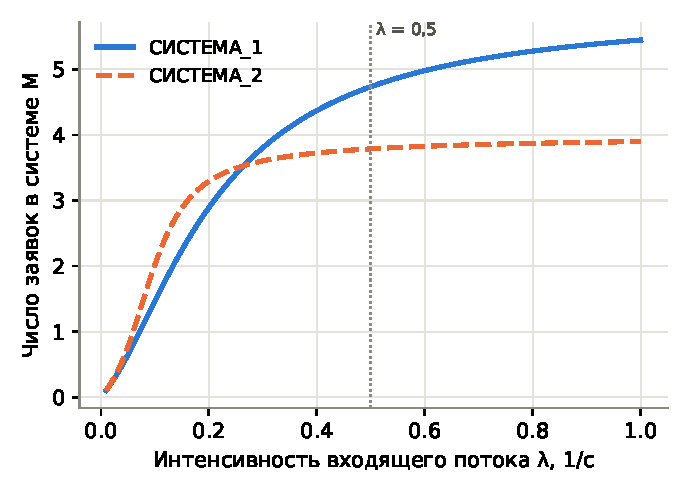
\includegraphics[width=\linewidth]{figures/m.pdf}\caption{Число заявок в системе}\label{fig:m}\end{subfigure}
\caption{Характеристики систем в зависимости от $\lambda$ (пунктир~--- заданное значение $\lambda = 0{,}5$)}
\end{figure}

Анализ графиков показывает:
\begin{itemize}
\item При малой интенсивности ($\lambda \lesssim 0{,}05$ 1/с) производительности систем практически совпадают
и равны $\lambda$, так как потери малы. С ростом $\lambda$ производительность СИСТЕМЫ\_2 быстро
насыщается на уровне $1/b = 0{,}1$ 1/с, а СИСТЕМЫ\_1 продолжает расти к пределу $0{,}2$ 1/с.
Таким образом, при любом $\lambda$ выполняется $\Lambda'_1 \ge \Lambda'_2$.
\item Вероятность потери в СИСТЕМЕ\_2 меньше только при $\lambda < 0{,}054$ 1/с (там общий накопитель на 3 места
эффективнее раздельных по 2), при большей интенсивности потери в СИСТЕМЕ\_1 ниже.
\item Загрузка прибора СИСТЕМЫ\_2 всегда выше: один прибор принимает весь поток, а в СИСТЕМЕ\_1
поток делится на два прибора.
\item Время пребывания в СИСТЕМЕ\_1 меньше при всех $\lambda$, разница растёт с нагрузкой.
\item Суммарная длина очередей и число заявок в СИСТЕМЕ\_1 больше, чем в СИСТЕМЕ\_2, при
$\lambda > 0{,}47$ и $\lambda > 0{,}26$ 1/с соответственно, так как суммарная ёмкость СИСТЕМЫ\_1 больше
(2 прибора + 4 места против 1 прибора + 3 мест). При заданном $\lambda=0{,}5$ это проявляется
незначительно превышением $L$.
\end{itemize}


\subsection{Влияние распределения заявок между приборами в СИСТЕМЕ\_1}
\begin{figure}[H]
\centering
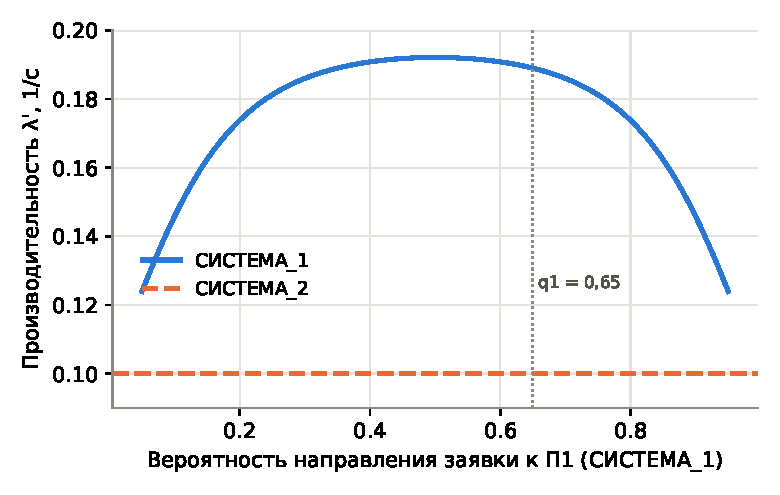
\includegraphics[width=0.6\textwidth]{figures/routing.pdf}
\caption{Производительность СИСТЕМЫ\_1 в зависимости от вероятности $q_1$}
\end{figure}
Максимальная производительность СИСТЕМЫ\_1 достигается при равномерном распределении заявок
($q_1 = 0{,}5$): \SoneSymThr\ 1/с. При заданном $q_1=0{,}65$ производительность ниже лишь на
$\approx 1{,}6\,\%$, при любом $q_1 \in [0{,}05;\,0{,}95]$ СИСТЕМА\_1 остаётся производительнее СИСТЕМЫ\_2.

% ======================= 9 =======================
\section{Выбор наилучшего варианта}
Критерий эффективности~--- \textbf{максимальная производительность системы} (интенсивность потока
обслуженных заявок $\Lambda'$).
\[
\Lambda'_1 = \SoneThr \ \text{1/с} \;>\; \Lambda'_2 = \StwoThr \ \text{1/с}.
\]
\textbf{Наилучшим вариантом является СИСТЕМА\_1} (два экспоненциальных прибора с раздельными
накопителями ёмкостью 2/2): её производительность в \Ratio\ раза выше. Кроме того, СИСТЕМА\_1 лучше и по
вероятности потерь, и по времени пребывания заявок; СИСТЕМА\_2 выигрывает только по загрузке
прибора и незначительно по суммарной длине очередей, что не относится к заданному критерию.
Вывод сохраняется при любой интенсивности входящего потока: при малых $\lambda$ производительности
систем совпадают, при росте $\lambda$ преимущество СИСТЕМЫ\_1 увеличивается.

% ======================= 10 =======================
\section{Заключение}
В работе построены марковские модели двух СМО: двухканальной системы с раздельными накопителями
(16 состояний) и одноканальной системы с эрланговским обслуживанием 3-го порядка (13 состояний,
метод фаз). Для каждой системы построены размеченные графы переходов и матрицы интенсивностей,
рассчитаны стационарные вероятности и полный набор характеристик через вероятности состояний,
корректность которых подтверждена фундаментальными соотношениями (формула Литтла и др.).
По критерию максимальной производительности выбрана СИСТЕМА\_1.

\appendix
\section*{Приложение А. Программа расчёта (Python)}
\addcontentsline{toc}{section}{Приложение А. Программа расчёта (Python)}
\lstinputlisting{code/model.py}

\end{document}
